\documentclass[a4paper,12pt]{report}
\usepackage[left=3cm,right=2.5cm,top=2.5cm,bottom=2.5cm]{geometry}
\usepackage[T1]{fontenc}
\usepackage[utf8]{inputenc}
\usepackage[english,greek]{babel}
\usepackage{amsmath,amsfonts,amssymb,amsthm}
\usepackage[parfill]{parskip}
\usepackage[unicode]{hyperref}
\usepackage{bookmark}
\usepackage{cite}
\usepackage{graphicx}
\usepackage{wrapfig}
\usepackage{subcaption}
\usepackage{float}
\usepackage{siunitx}
\usepackage{color}
\usepackage{kmath,kerkis}
\usepackage{url}
\usepackage{hyperref}
\usepackage{tikz}
\usepackage[ruled,nosemicolon,linesnumbered]{algorithm2e}
\let\oldnl\nl% Store \nl in \oldnl
\newcommand{\nonl}{\renewcommand{\nl}{\let\nl\oldnl}}% Remove line number for one line


\graphicspath{{../graphics/}}

\def\tl{\textlatin}
\def\tg{\textgreek}

\newtheorem{definition}{Ορισμός}
\newtheorem{lemma}{Λήμμα}

\def\bigO{\mathcal{O}}

\begin{document}

\begin{titlepage}

\begin{figure}[H]
  \begin{center}
    \includegraphics[width=3cm]{auth.pdf}
    \label{fig:cover_auth_logo}
  \end{center}
\end{figure}

\centering
\Large Αριστοτέλειο Πανεπιστήμιο Θεσσαλονίκης\\
\Large Πολυτεχνική Σχολή\\
\large Τμήμα Ηλεκτρολόγων Μηχανικών και Μηχανικών Υπολογιστών\\
\large Τομέας Ηλεκτρονικής και Υπολογιστών

\vspace{\fill}

\LARGE Υπολογισμός της Ευκλείδειας Απόστασης δύο Τριγωνικών Πλεγμάτων

\vspace{\fill}

\Large Διπλωματική Εργασία\\
\Large Καρελής Παναγιώτης

\vspace{\fill}
\raggedright

\begin{tabular}{ll}
\textbf{Επιβλέπων:} & Πιτσιάνης Νικόλαος\\
 & Αναπληρωτής Καθηγητής Α.Π.Θ.\\
\end{tabular}

\centering
\vspace{\fill}
\today

\end{titlepage}

\begin{abstract}
Άδειο
\end{abstract}

\selectlanguage{english}
\begin{abstract}
Empty
\end{abstract}

\thispagestyle{empty}

\selectlanguage{greek}

\section*{Ευχαριστίες}
\thispagestyle{empty}

Άδειο

\clearpage


\title{Υπολογισμός της Ευκλείδειας Απόστασης δύο Τριγωνικών Πλεγμάτων}
\author{Παναγιώτης Καρελής \\
\href{mailto:karelisp@ece.auth.gr}{\tl{karelisp@ece.auth.gr}}}
\maketitle

\tableofcontents
\thispagestyle{empty}

\chapter{Εισαγωγή}
\label{ch:introduction}
\section{Κίνητρο}

\section{Περιγραφή του Προβλήματος}

\section{Στόχοι της Διπλωματικής Εργασίας}

\section{Διάρθρωση της Διπλωματικής Εργασίας}
Στο \textbf{Κεφάλαιο \ref{ch:introduction}} έγινε μια εισαγωγή στο 
πρόβλημα υπολογισμού της απόστασης δύο πλεγμάτων και παρουσιάστηκαν
τα κίνητρα που οδήγησαν στην υλοποίηση των αλγορίθμων που θα 
παρουσιαστούν. 

Στο \textbf{Κεφάλαιο \ref{ch:theoretical_background}} παρουσιάζεται το 
θεωρητικό υπόβαθρο που απαιτείται από τον αναγνώστη ώστε να κατανοήσει
πλήρως το πρόβλημα και την προτεινόμενη λύση.

Στο \textbf{Κεφάλαιο \ref{ch:related_work}} αναφέρεται η σχετική 
βιβλιογραφία, δηλαδή πώς αντιμετώπισαν άλλοι ερευνητές το ίδιο ή 
παρόμοια προβλήματα. 
Παρουσιάζονται επίσης ομοιότητες και διαφορές
των υπολοίπων προσεγγίσεων σε σχέση με τη δική μας.

Στο \textbf{Κεφάλαιο \ref{ch:methodology}} αναλύεται η μεθοδολογία 
που προτείνουμε και παρουσιάζεται η υλοποίηση των αλγορίθμων μας.

Στο \textbf{Κεφάλαιο \ref{ch:experiments}} παρατίθενται τα αποτελέσματα 
από τα πειράματα που εκτελέσαμε. 
Οι μετρήσεις των πειραμάτων περιλαμβάνουν την εκτίμηση της συνάρτησης 
κόστους που ορίζεται στην ενότητα \ref{sec:cost_metric} καθώς και τους χρόνους
εκτέλεσης των αλγορίθμων. 

Στο \textbf{Κεφάλαιο \ref{ch:future_work}} σχολιάζονται τα αποτελέσματα
και παρουσιάζονται σκέψεις για μελλοντική επέκταση και βελτίωση των 
ιδεών της παρούσας διπλωματικής εργασίας.

\chapter{Θεωρητικό Υπόβαθρο}
\label{ch:theoretical_background}

\section{Πλέγματα}
\begin{wrapfigure}{r}{0.25\textwidth}
    \centering
    \includegraphics[width=0.25\textwidth]{Dolphin_triangle_mesh.png}
    \caption[Παράδειγμα Τριγωνικού Πλέγματος]{
        Παράδειγμα τριγωνικού πλέγματος που αναπαριστά ένα δελφίνι.
    }
    \label{fig:example_mesh}
\end{wrapfigure}
\label{sec:triangle_meshes}
Στην Υπολογιστική Γεωμετρία τα πλέγματα αποτελούν την αναπαράσταση
μιας μεγαλύτερης γεωμετρικής περιοχής από μικρότερα διακριτά στοιχεία.
Τα πλέγματα χρησιμοποιούνται συνήθως για τον υπολογισμό λύσεων μερικών 
διαφορικών εξισώσεων, για την απόδοση γραφικών υπολογιστών, και για
ανάλυση γεωγραφικών και χαρτογραφικών δεδομένων.
Ένα πλέγμα χωρίζει τον χώρο σε μικρότερα στοιχεία (πολύγωνα ή πολύεδρα) όπου
μπορούν να λυθούν οι εξισώσεις, το οποίο στη συνέχεια προσεγγίζει τη λύση 
στο ευρύτερο πεδίο. 
Τα πλέγματα που αποτελούνται από πολύεδρα αντιπροσωπεύουν ρητά τόσο την 
επιφάνεια όσο και τον όγκο ενός αντικειμένου, ενώ τα πολυγωνικά 
πλέγματα αντιπροσωπεύουν μόνο την επιφάνεια (ο όγκος υπονοείται).
Για το πρόβλημα υπολογισμού της Ευκλείδειας απόστασης, ενδιαφερόμαστε 
μόνο για την εξωτερική επιφάνεια των αντικειμένων του τρισδιάστατου χώρου. 

Ένας τύπος πολυγωνικών πλεγμάτων είναι τα τριγωνικά πλέγματα 
(σχήμα \ref{fig:example_mesh}).
Αποτελούνται από ένα σύνολο τριγώνων στις τρεις διαστάσεις, 
τα οποία συνδέονται με τις κοινές τους ακμές ή κορυφές. 
Γεωμετρικά, ένα πλέγμα είναι μια τμηματικά επίπεδη επιφάνεια.
Η τελευταία ιδιότητα ισχύει πάντοτε για τα τριγωνικά πλέγματα.

Υπάρχουν διάφοροι τρόποι για την αποθήκευση ενός τριγωνικού πλέγματος 
στη μνήμη του υπολογιστή. 
Υπάρχουν επίσης μέθοδοι μετατροπής του ενός 
τρόπου αποθήκευσης σε έναν άλλο.
Ενδεικτικά αναφέρουμε την αποθήκευση με:
\begin{itemize}
    \item \textbf{Σετ τριγώνων}: 
    Το πλέγμα αναπαρίσταται απλά από τα τρίγωνα 
    του. 
    Δηλαδή αποθηκεύονται οι συντεταγμένες των κορυφών κάθε τριγώνου.
    \item \textbf{Σετ Τριγώνων με δείκτες}: 
    Το πλέγμα αναπαρίσταται από ένα σετ
    κόμβων και ένα σετ από τριπλέτες με δείκτες στους κόμβους.
    Η κάθε τριπλέτα αναπαριστά ένα τρίγωνο.
    \item \textbf{Λωρίδες Τριγώνων}: 
    Η αποθήκευση αυτή βασίζεται στο γεγονός ότι 
    δύο γειτονικά τρίγωνα μοιράζονται τη μία τους πλευρά. Αυτός 
    ο τρόπος χρησιμοποιείται για συμπίεση των πλεγμάτων.
    \item \textbf{Δομή Τρίγωνου-Γείτονα}: 
    Υποστηρίζει ερωτήματα γειτνίασης τριγώνων.
    \item \textbf{Δομή \tl{Winged-Edge}}: 
    Αποθηκεύει δεδομένα κόμβων, ακμών και όψεων.
    Επιτρέπει εύκολη διάβαση στο πλέγμα μεταξύ όψεων, ακμών και κορυφών.
\end{itemize} 
Για τους αλγορίθμους που περιγράφουμε παρακάτω αρκεί ο πρώτος τρόπος 
αναπαράστασης. 

Τέλος, για τις διάφορες εφαρμογές που χρησιμοποιούνται, τα πλέγματα 
χαρακτηρίζονται και από την ποιότητα τους. Οι πιο συνηθισμένες μετρικές 
ποιότητας είναι:
\begin{itemize}
    \item \textbf{Λοξότητα (\tl{Skewness})}: \\
    Η λοξότητα είναι ο λόγος της απόκλισης μεταξύ του βέλτιστου μεγέθους
    στοιχείου προς στο υπάρχον μέγεθος στοιχείου. 
    Το εύρος της λοξότητας είναι μεταξύ 0 (ιδανικό) έως 1 (χειρότερο).
    Τα πολύ λοξά στοιχεία δεν προτιμώνται λόγω της κακής ακρίβειας 
    που προκαλούν στις παρεμβαλλόμενες περιοχές.
    Ανάλογα με το στοιχείο (τρίγωνο, τετράπλευρο, τετράεδρο, 
    εξάεδρο κλπ) διαφοροποιείται μαθηματικός τύπος 
    για τον υπολογισμό της λοξότητας.

    \item \textbf{Ομαλότητα (\tl{Smoothness})}: \\
    Η αλλαγή στο μέγεθος των στοιχείων πρέπει να είναι ομαλή. 
    Συνήθως αποφεύγονται ξαφνικά άλματα στο μέγεθος των στοιχείων γιατί αυτό 
    μπορεί να προκαλέσει λανθασμένα αποτελέσματα σε κοντινούς κόμβους.
    
    \item \textbf{Αναλογία Διαστάσεων (\tl{Aspect Ratio})}: \\
    Εν συντομία, ο λόγος διαστάσεων είναι ο λόγος του μεγαλύτερου μήκους 
    ενός στοιχείου προς το μικρότερο μήκος. 
    Ο ιδανικός λόγος διαστάσεων είναι 1. 
    Όσο μικρότερος είναι, τόσο υψηλότερη είναι η ποιότητα ενός στοιχείου. 
    Η μέθοδος υπολογισμού ποικίλλει ανάλογα με τον τύπο κελιού.
\end{itemize}

Σε πραγματικές εφαρμογές, τα πλέγματα συνήθως σχεδιάζονται έτσι ώστε 
να μην παραβιάζουν σε μεγάλο βαθμό τις παραπάνω μετρικές ποιότητας.
Αυτή η παρατήρηση είναι χρήσιμη για τον σχεδιασμό της δομής δεδομένων 
που προτείνουμε.

\begin{figure}[h]
    \centering
    \includegraphics[width=0.45\textwidth]{airplane_bad_mesh.png}
    \includegraphics[width=0.45\textwidth]{airplane_good_mesh.png}
    \caption[Παράδειγμα Ποιότητας Πλεγμάτων]{
        Παράδειγμα Ποιότητας Πλεγμάτων - Και τα δύο πλέγματα 
        αναπαριστούν το ίδιο αεροπλάνο. Το δεξί πλέγμα είναι 
        καλύτερης ποιότητας από το αριστερό που φαίνεται να 
        παραβιάζει όλα τα κριτήρια ποιότητας που αναφέρθηκαν
        (\tl{skweness, smoothness, aspect ratio}).
    }
\end{figure}




\section{Ευρετήρια για Χωρικά Δεδομένα}

\section{Οριοθετικοί Όγκοι}
\subsection{Οριοθετικά Πλαίσια Ευθυγραμμισμένα με τους Άξονες}

\section{Ιεραρχίες Οριοθετικών Όγκων}

\chapter{Σχετική Βιβλιογραφία}
\label{ch:related_work}
Τα ερωτήματα εγγύτητας και η ανίχνευση σύγκρουσης διερευνώνται 
εκτενώς για δεκαετίες από ερευνητές στα γραφικά υπολογιστών, στη ρομποτική,
στις προσομοίωσες, την υπολογιστική γεωμετρία και τα κινούμενα σχέδια 
υπολογιστών. 
Εκτός από την ανίχνευση σύγκρουσης και τον υπολογισμό απόστασης, υπάρχει
σημαντική βιβλιογραφία σχετική με τις Ιεραρχίες Οριοθετικών Όγκων 
(\tl{BVH}) και τις διάφορες εφαρμογές τους. 
Σε αυτό το κεφάλαιο κάνουμε αναφορά σε άρθρα της βιβλιογραφίας 
που μελετούν το ίδιο ή παρόμοιο πρόβλημα με το δικό μας
και επισημαίνουμε τις τεχνικές που χρησιμοποιούνται 
και στη δική μας μεθοδολογία.

\section{Εύρεση Κοντινότερου Σημείου σε ένα Σύνολο Σημείων}

\section{Ανίχνευση Σύγκρουσης και Υπολογισμός Απόστασης Πολυγώνων}
% να πω για linear programming 
% These include Dobkin-
% Kirkpatrick hierarchies [DK82], linear programming [Sei90] and algorithms for intersecting
% convex p olytop es [Cha89 ] 
% και γενικά ό,τι αναφέρεται στο paper του GJK.

\section{Ιεραρχικές Δομές Δεδομένων}
%να αναφέρω SAH
%R-Trees
%BSP Trees
% Απόσταση Σημείου από Πολυγωνικό Πλέγμα
% Απόσταση Δύο Πολυγωνικών Πλεγμάτων
% Απόσταση Αντικειμένων που Περιγράφονται από \tl{NURBS}

\chapter{Μεθοδολογία}
\label{ch:methodology}

Σε αυτή την εργασία κάνουμε την υπόθεση ότι τα αντικείμενα του 
τρισδιάστατου χώρου αναπαρίστανται από την εξωτερική τους επιφάνεια 
η οποία περιγράφεται από τριγωνικά πλέγματα. 
Αυτή η υπόθεση δεν είναι περιοριστική, καθώς η προσαρμογή της μεθοδολογίας 
που ακολουθούμε σε περιγραφές άλλου τύπου δεν είναι δύσκολη.
Για την εφαρμογή της μεθοδολογίας θα πρέπει:
\begin{enumerate}
    \item Είτε οι αναπαραστάσεις διαφορετικού τύπου να μετατραπούν σε αναπαράσταση 
    με τριγωνικό πλέγμα (αυτή η μετατροπή είναι πάντοτε εφικτή, για παράδειγμα, 
    από πολυγωνικά πλέγματα).
    \item Είτε να δοθούν δύο ρουτίνες για τα στοιχεία από τα οποία αποτελείται η 
    αναπαράσταση. Η μία να υπολογίζει το \tl{AABB} του στοιχείου 
    ενώ η άλλη να υπολογίζει την Ευκλείδεια απόσταση δύο τέτοιων στοιχείων.
\end{enumerate}
Επιπλέον, σημειώνουμε ότι η χρήση επιφανειακών αναπαραστάσεων για τα αντικείμενα 
υπονοεί πως δε θα γίνει ανίχνευση σύγκρουσης εάν το ένα αντικείμενο περικλείει 
εντελώς το άλλο, αλλά τέτοιες καταστάσεις αποφεύγονται σε πολλές εφαρμογές.


\section{Στοιχειώδεις Γεωμετρικές Πράξεις}
\subsection{Ευκλείδεια Απόσταση δύο Τριγώνων}
\label{subsec:tria_distance}
% Έστω τα τρίγωνα $P$ και $Q$ στον $\mathbb{R}^3$.
% Η Ευκλείδεια απόσταση $d(P,Q)$ μεταξύ των τριγώνων $P$ και $Q$
% ορίζεται ως:
% \[ d(P,Q) = \min_{p \in P, q \in Q} |p - q| \]
% όπου με $|p-q|$ συμβολίζεται η Ευκλείδεια απόσταση των σημείων 
% $p$ και $q$.

% Έστω p,q

\subsubsection{Ευκλείδεια Απόσταση δύο Ευθυγράμμων Τμημάτων}
\subsubsection{Ευκλείδεια Απόσταση Σημείου και Τριγώνου}

\subsection{Γεωμετρικές Πράξεις για \tl{AABB}}
Ένα οριοθετικό πλαίσιο ευθυγραμμισμένο με τους άξονες (\tl{AABB})
είναι, απλώς, ένα ορθογώνιο παραλληλεπίπεδο του οποίου οι 
έδρες είναι κάθετες σε ένα από τα διανύσματα βάσης.

Ένα \tl{AABB} αναπαριστάται στη μνήμη από τα άκρα της κύριας 
διαγωνίου του.
Δηλαδή το σημείο $S$ με τις μικρότερες $x$, $y$, $z$ συντεταγμένες
και το σημείο $T$ με τις μεγαλύτερες $x$, $y$, $z$ συντεταγμένες.

\begin{figure}[h]
    \centering
    
    \newcommand{\Depth}{2}
    \newcommand{\Height}{2}
    \newcommand{\Width}{3}
    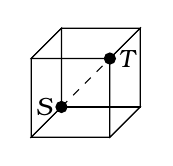
\begin{tikzpicture}
        \coordinate (O) at (0,0,0);
        \coordinate (A) at (0,\Width,0);
        \coordinate (B) at (0,\Width,\Height);
        \coordinate (C) at (0,0,\Height);
        \coordinate (D) at (\Depth,0,0);
        \coordinate (E) at (\Depth,\Width,0);
        \coordinate (F) at (\Depth,\Width,\Height);
        \coordinate (G) at (\Depth,0,\Height);

        \draw[] (O) -- (C) -- (G) -- (D) -- cycle;% Bottom Face
        \draw[] (O) -- (A) -- (E) -- (D) -- cycle;% Back Face
        \draw[] (O) -- (A) -- (B) -- (C) -- cycle;% Left Face
        \draw[] (D) -- (E) -- (F) -- (G) -- cycle;% Right Face
        \draw[] (C) -- (B) -- (F) -- (G) -- cycle;% Front Face
        \draw[] (A) -- (B) -- (F) -- (E) -- cycle;% Top Face

        \draw[fill=black] (O) circle (2pt) node[left]{$S$};
        \draw[fill=black] (F) circle (2pt) node[right]{$T$};
        \draw[dashed] (O) -- (F);
    \end{tikzpicture}
    \caption[Αναπαράσταση ενός \tl{AABB}]{Αναπαράσταση ενός \tl{AABB}}
\end{figure}

\subsubsection{Υπολογισμός Απόστασης \tl{AABB-AABB}}
Έστω τα ευθυγραμμισμένα με τους άξονες πλαίσια
$P$ και $Q$ στον $\mathbb{R}^3$.
Η Ευκλείδεια απόσταση $d(P,Q)$ μεταξύ των πλαισίων $P$ και $Q$
ορίζεται ως:
\[ d(P,Q) = \min_{p \in P, q \in Q} \lVert p - q \rVert \]
όπου με $\lVert p - q \rVert$ συμβολίζεται η Ευκλείδεια 
απόσταση των σημείων $p$ και $q$.

Για τον υπολογισμό της απόστασης μεταξύ δύο τέτοιων πλαισίων, 
εκμεταλλευόμαστε το γεγονός ότι οι πλευρές τους είναι ευθυγραμμισμένες
με του άξονες.
Έτσι μπορούμε να υπολογίσουμε την απόσταση χωρίζοντας τη στις συνιστώσες της.
Τελικά, προκύπτει ο αλγόριθμος \ref{alg:aabb_dist}, 
όμοιος με αυτόν που περιγράφεται στο \cite{krishnamurthy2011gpu}.
Στον παραπάνω αλγόριθμο  ο τελεστής "$-$" στις γραμμές 
$1$,$2$ είναι διανυσματική αφαίρεση των συντεταγμένων των σημείων.
Ο τελεστής \tl{\texttt{max(0, $v$)}} είναι επίσης διανυσματικός και
αντικαθιστά όλες τις αρνητικές τιμές ενός διανύσματος $v$
με $0$.
Ο τελεστής $\cdot$ είναι το εσωτερικό γινόμενο διανυσμάτων.

\selectlanguage{english}
\IncMargin{1.5em}
\begin{algorithm}[H]
    \label{alg:aabb_dist}
    \caption[Υπολογισμός Απόστασης δύο \tl{AABB}]{
        \tg{Υπολογισμός της Ευκλείδειας Απόστασης δύο AABB}
    }
    \DontPrintSemicolon
    \KwIn{Two AABBs $P$, $Q$}
    \KwOut{Euclidean Distance of $P$ and $Q$}
    \SetKwFunction{funcname}{AABB\_distance}
    \SetKwFunction{max}{max}
    \Indm\nonl\funcname($P$, $Q$)\\
    \Indp
        $w \gets \max(0, P.S - Q.T)$\;
        $v \gets \max(0, Q.S - P.T)$\;
        \Return{$\sqrt{v \cdot v + w \cdot w}$}

    
\end{algorithm}
\DecMargin{1.5em}
\selectlanguage{greek}

\subsubsection{Κατασκευή \tl{AABB} Από Τρίγωνο}
Με τον αλγόριθμο \ref{alg:aabb_from_triangle} κατασκευάζουμε 
ένα \tl{AABB} που εξ' ολοκλήρου περικλείει ένα τρίγωνο.
Η ρουτίνα \tl{\texttt{vertices($T$)}} επιστρέφει τις 
τρεις κορυφές του τριγώνου $T$.
Οι τελεστές \tl{\texttt{min(), max()}} είναι διανυσματικοί,
δέχονται ως όρισμα μια λίστα από διανύσματα και επιστρέφουν 
ένα διάνυσμα με τις ελάχιστες/μέγιστες συντεταγμένες ανά άξονα.

\selectlanguage{english}
\IncMargin{1.5em}
\begin{algorithm}[H]
    \label{alg:aabb_from_triangle}
    \caption[Κατασκευή \tl{AABB} από Τρίγωνο]{
        \tg{Κατασκευή \tl{AABB} από Τρίγωνο}
    }
    \DontPrintSemicolon
    \KwIn{A Triangle $T$}
    \KwOut{An AABB Enclosing $T$}
    \SetKwFunction{funcname}{AABB}
    \SetKwFunction{min}{min}
    \SetKwFunction{max}{max}
    \SetKwFunction{vertices}{vertices}
    \Indm\nonl\funcname($T$)\\
    \Indp
        $S \gets \min(\vertices(T))$\;
        $T \gets \max(\vertices(T))$\; 
        \Return{ \{$S$, $T$\}}
    
\end{algorithm}
\DecMargin{1.5em}
\selectlanguage{greek}

\subsubsection{Συνένωση Δύο \tl{AABB}}
Ο αλγόριθμος \ref{alg:combine_aabbs} κατασκευάζει ένα \tl{AABB} περικλείει
εξ' ολοκλήρου δύο άλλα \tl{AABB} που δέχεται ως ορίσματα. 
Αυτή η πράξη είναι χρήσιμη γιατί αν έχουμε ήδη βρει τα \tl{AABB} για δύο 
ομάδες αντικειμένων ξεχωριστά, μπορούμε σε σταθερό χρόνο $\bigO(1)$ να 
κατασκευάσουμε το \tl{AABB} που περικλείει όλα τα αντικείμενα. 
Οι τελεστές \tl{\texttt{min(), max()}} είναι ίδιοι με πριν.

\selectlanguage{english}
\IncMargin{1.5em}
\begin{algorithm}[H]
    \label{alg:combine_aabbs}
    \caption[Κατασκευή \tl{AABB} από δύο άλλα \tl{AABB}]{
        \tg{Κατασκευή \tl{AABB} από δύο άλλα \tl{AABB}}
    }
    \DontPrintSemicolon
    \KwIn{Two AABBs $P$, $Q$}
    \KwOut{An AABB Enclosing $P$ and $Q$}
    \SetKwFunction{funcname}{combine\_AABB}
    \Indm\nonl\funcname($P$, $Q$)\\
    \Indp
        
    $S \gets \min(P.S, Q.S)$\;
    $T \gets \max(P.T, Q.T)$\; 
    \Return{ \{$S$, $T$\}}
\end{algorithm}
\DecMargin{1.5em}
\selectlanguage{greek}

\section{Αλγόριθμοι Εξαντλητικής Αναζήτησης}
\label{sec:exhaustive_search}
Έστω δύο αντικείμενα του τρισδιάστατου χώρου που αναπαρίστανται από 
τριγωνικά πλέγματα.
Από τον ορισμό της Ευκλείδειας απόστασης δύο τριγωνικών πλεγμάτων που
δόθηκε στην ενότητα \ref{sec:problem_description} και τη χρήση μιας 
ρουτίνας \tl{\texttt{triangle\_distance(p, q)}}, προκύπτει ο 
τετριμμένος αλγόριθμος \ref{alg:exhaustive_search}. 
Η πολυπλοκότητα του αλγορίθμου είναι $\bigO(N*M)$, όπου 
$N$ και $M$ είναι το πλήθος των τριγώνων των δύο αντικειμένων.

\selectlanguage{english}
\IncMargin{1.5em}
\begin{algorithm}[h]

    \caption[Απόσταση Τριγωνικών Πλεγμάτων με Πλήρη Αναζήτηση]{
        \tg{Απόσταση Τριγωνικών Πλεγμάτων με Πλήρη Αναζήτηση}
    }
    \label{alg:exhaustive_search}
    \DontPrintSemicolon
    \KwIn{Two Triangle Meshes $P$, $Q$}
    \KwOut{Euclidean Distance of $P$ and $Q$}
    \SetKwFunction{dist}{triangle\_distance}
    \SetKwFunction{trias}{triangles}
    \SetKwFunction{min}{min}
    \SetKwFunction{exhaustivesearch}{triangle\_mesh\_distance}
    \Indm\nonl\exhaustivesearch ($P$, $Q$)\\
    \Indp
        $T_P \gets$ \trias($P$) \;
        $T_Q \gets$ \trias($Q$) \; 
        $distance \gets \inf$ \;
        \ForEach{$p \in T_P$}{
            \ForEach{$q \in T_Q$}{
                $distance \gets \min(distance, \dist(p,q))$\;
            }
        }
        \Return{$distance$}
\end{algorithm}
\DecMargin{1.5em}
\selectlanguage{greek}

Σύμφωνα με τη μελέτη που έγινε στην ενότητα \ref{sec:bounding_volumes}
μπορούμε να επιταχύνουμε τον χρόνο εκτέλεσης του αλγορίθμου αν 
χρησιμοποιήσουμε οριοθετικούς όγκους.
Συγκεκριμένα, θα χρησιμοποιήσουμε Οριοθετικά Πλαίσια Ευθυγραμμισμένα 
με τους Άξονες (\tl{AABB}). 
Όπως φαίνεται από τον πίνακα της ενότητας \ref{sec:geom_tests_cost},
ο υπολογισμός της ελάχιστης απόστασης \textit{\tl{AABB - AABB}} είναι πολύ πιο 
"οικονομικός" υπολογιστικά σε σχέση με τον υπολογισμό της απόστασης 
\textit{τρίγωνο - τρίγωνο}.
Μπορούμε να εκμεταλλευτούμε αυτό το γεγονός και σε συνδυασμό με το παρακάτω λήμμα 
να σχεδιάσουμε έναν ταχύτερο αλγόριθμο.

\begin{lemma}
    Έστω δύο σύνολα $S_A$ και $S_B$ που αποτελούνται από χωρικά αντικείμενα. 
    Έστω οι οριοθετικοί όγκοι $BV_A$ και $BV_B$ που εξ' ολοκλήρου περικλείουν 
    τα αντικείμενα των σύνολων  $S_A$ και $S_B$, αντίστοιχα. Τότε:
    
    \[ distance(BV_A, BV_B) \leq distance(a, b) , 
    \forall a \in S_A, \forall b \in S_B \]

    Δηλαδή, η Ευκλείδεια απόσταση οποιουδήποτε ζεύγους αντικειμένων από τα δύο σύνολα 
    θα είναι μεγαλύτερη ή ίση με την Ευκλείδεια απόσταση των οριοθετικών όγκων 
    των συνόλων.
    \label{lemma:box_distance}
\end{lemma}


\begin{proof}
    Συμβολίζουμε με $BV_A$ το σύνολο των σημείων του 
    οριοθετικού όγκου, $BV_A$. 
    Όμοια και για το σύνολο $BV_B$.

    Επίσης, έχουμε
    $S_A = \bigcup\limits_{a \in S_A} a $ και $S_B = \bigcup\limits_{b \in S_B} b$,
    όπου με $a$, $b$ συμβολίζουμε το σύνολο των σημείων των 
    χωρικών αντικειμένων $a$ και $b$.

    Αφού οι οριοθετικοί όγκοι περικλείουν τα σύνολα των 
    αντικειμένων $S_A$ και $S_B$ ισχύει επίσης ότι 
    $S_A \subseteq BV_A $ και 
    $S_B \subseteq BV_B $.

    Έστω ότι υπάρχουν αντικείμενα $a \in S_A$, $b \in S_B$ με απόσταση μικρότερη 
    από αυτή των οριοθετικών όγκων. Τότε, υπάρχουν σημεία $p \in a \subseteq S_A 
    \subseteq BV_A$ και $q \in b \subseteq S_B \subseteq BV_A$ ώστε 
    \[\lVert p - q \rVert < distance(BV_A, BV_B)\]
    Από τον ορισμό της Ευκλείδειας απόστασης δύο οριοθετικών όγκων καταλήγουμε 
    σε άτοπο.
\end{proof}

Προκύπτει, λοιπόν, ο αλγόριθμος \ref{alg:exhaustive_search_aabb}.
Αρχικά, κάθε τρίγωνο περικλείεται από 
ένα \tl{AABB}. Σε κάθε βήμα του αλγορίθμου είναι γνωστή η μικρότερη απόσταση 
που έχει υπολογιστεί μέχρι εκείνη τη στιγμή. Έτσι, για κάθε ζεύγος τριγώνων, 
πρώτα γίνεται ο γρήγορος υπολογισμός απόστασης \tl{AABB-AABB} και μόνο όταν αυτή 
η απόσταση είναι μικρότερη από την τρέχουσα απόσταση γίνεται ο έλεγχος 
τρίγωνο-τρίγωνο.
Η υπολογιστική πολυπλοκότητα παραμένει $\bigO(N*M)$, όπως και πριν.
Σημειώνεται, ότι ο χρόνος εκτέλεσης επηρεάζεται από τη σειρά που θα γίνουν 
οι πράξεις. Δηλαδή αν η μικρότερη απόσταση βρεθεί από πολύ νωρίς, τότε 
θα γίνουν πολύ λίγοι υπολογισμοί τρίγωνο-τρίγωνο, ενώ το αντίθετο θα συμβεί 
αν η μικρότερη απόσταση βρεθεί πιο αργά.

\selectlanguage{english}
\IncMargin{1.5em}
\begin{algorithm}[h]
    \caption[Απόσταση Τριγωνικών Πλεγμάτων με Πλήρη Αναζήτηση και \tl{AABB}]{
        \tg{Απόσταση Τριγωνικών Πλεγμάτων με Πλήρη Αναζήτηση και} AABB
        }
    \label{alg:exhaustive_search_aabb}
    \DontPrintSemicolon
    \KwIn{Two Triangle Meshes $P$, $Q$}
    \KwOut{Euclidean Distance of $P$ and $Q$}
    \SetKwFunction{dist}{triangle\_distance}
    \SetKwFunction{aabbdist}{AABB\_distance}
    \SetKwFunction{trias}{triangles}
    \SetKwFunction{min}{min}
    \SetKwFunction{aabb}{AABB}
    \SetKwFunction{funcname}{triangle\_mesh\_distance}
    \Indm\nonl\funcname($P$, $Q$)\\
    \Indp
        $T_P \gets$ \trias($P$) \;
        $T_Q \gets$ \trias($Q$) \;
        precalculate AABBs of $T_P$\;
        precalculate AABBs of $T_Q$\; 
        $distance \gets \inf$ \;
        \ForEach{$p \in T_P$}{
            \ForEach{$q \in T_Q$}{
                \If{\aabbdist(\aabb($p$), \aabb($q$)) $ < distance$}{
                    $distance \gets \min(distance, \dist(p,q))$\;
                }
            }
        }
        \Return{$distance$}
\end{algorithm}
\DecMargin{1.5em}
\selectlanguage{greek}

Παραπάνω, θα μπορούσαμε να χρησιμοποιήσουμε οποιονδήποτε τύπο οριοθετικού όγκου.
Οι λόγοι για τους οποίους γίνεται η επιλογή των \tl{AABB} είναι:
\begin{enumerate}
    \item Η Ιεραρχία Οριοθετικών Όγκων που σχεδιάζουμε και προτείνουμε 
    στην ενότητα \ref{sec:design_bvh} χρησιμοποιεί επίσης \tl{AABB}.
    Επομένως, μπορεί να υπάρξει ένα μέτρο σύγκρισης μεταξύ των 
    αλγορίθμων.
    \item Η κατασκευή ενός \tl{AABB} 
    που περικλείει εξ' ολοκλήρου ένα τρίγωνο και έχει ελάχιστο όγκο 
    είναι εύκολη (αλγόριθμος \ref{alg:aabb_from_triangle}).
    \item Ο υπολογισμός της Ευκλείδειας απόστασης 
    δύο \tl{AABB} (αλγόριθμος \ref{alg:aabb_dist}) είναι 
    εύκολος (αλγόριθμος \ref{alg:aabb_dist}).
    \item Η συνένωση δύο \tl{AABB} για την κατασκευή 
    ενός μεγαλύτερου που περικλείει και τα δύο είναι επίσης 
    εύκολη (αλγόριθμος \ref{alg:combine_aabbs}). 
    Η συνένωση είναι χρήσιμη πράξη για την κατασκευή της 
    ιεραρχίας. 
\end{enumerate}

\section{Ορισμός Μετρικής Κόστους Αναζήτησης}
\label{sec:cost_metric}

Σε αυτήν την ενότητα, ορίζουμε μια μετρική κόστους αναζήτησης
ώστε να μπορούμε να συγκρίνουμε την επίδοση των αλγορίθμων που μελετώνται.
Η ίδια μετρική χρησιμοποιείται και στα \cite{gottschalk1996obbtree},
\cite{larsen1999fast} για τη σύγκριση διάφορων ιεραρχικών δομών δεδομένων.
Δοθέντος δύο αντικειμένων, το συνολικό κόστος για τον υπολογισμό της μεταξύ τους 
Ευκλείδειας απόστασης μπορεί να δοθεί από την ακόλουθη εξίσωση κόστους:

\[ T = N_v \times C_v + N_p \times C_p \]

Όπου 
\begin{description}
    \item[$T$] το συνολικό κόστος για τον υπολογισμό της απόστασης,
    \item[$N_v$] το πλήθος των υπολογισμών απόστασης μεταξύ οριοθετικών όγκων,
    \item[$C_v$] το κόστος υπολογισμού απόστασης μεταξύ οριοθετικών όγκων,
    \item[$N_p$] το πλήθος των υπολογισμών απόστασης μεταξύ των \tl{primitives}
    \footnote{\tl{Geometric primitives} είναι κάποια απλά γεωμετρικά σχήματα 
    που μπορεί να χειριστεί ένα σύστημα. Συνήθως είναι σημεία, πολύγωνα, πολύεδρα κλπ.}
    \item[$C_p$] το κόστος υπολογισμού απόστασης μεταξύ των \tl{primitives}
\end{description}

Η επιλογή του τύπου οριοθετικού όγκου που θα χρησιμοποιηθεί, κατά τη σχεδίαση μιας 
ιεραρχίας, διέπεται από δύο αντικρουόμενους περιορισμούς\footnote{
    Στις ενότητες \ref{sec:bounding_volumes}, \ref{sec:bvh}, γίνεται 
    λεπτομερέστερη περιγραφή για αυτό το \tl{trade-off} 
}:
\begin{enumerate}
    \item Θα πρέπει να ακολουθεί το μοντέλο όσο πιο στενά γίνεται (\tl{tight-fit})
    για να μειωθούν οι τιμές $N_v$, $N_p$.
    \item Ο υπολογισμός της απόστασης μεταξύ οριοθετικών όγκων να είναι όσο το 
    δυνατόν ταχύτερος (για να μειωθεί το κόστος $C_v$)
\end{enumerate}

Για αυτή την εργασία οι οριοθετικοί όγκοι είναι \tl{AABB}, ενώ τα \tl{primitives} 
είναι τρίγωνα.
Τα κόστη $C_v$, $C_p$ δίνονται στους πίνακες της ενότητας \ref{sec:geom_tests_cost}.
Οι τιμές των $N_v$, $N_p$ μετρώνται πειραματικά ανάλογα με τα δεδομένα εισόδου 
(γεωμετρία, μέγεθος, προσανατολισμό, ποιότητα των πλεγμάτων).


Σημείωση: στην παραπάνω μετρική κόστους δεν προσμετράται το κόστος προεπεξεργασίας 
των δεδομένων (πχ για την κατασκευή μιας ιεραρχίας).
Το συνολικό κόστος (προ-επεξεργασία και αναζήτηση) "συμπεριλαμβάνεται" στη
μέτρηση των χρόνων εκτέλεσης των πειραμάτων.


\section{Σχεδιασμός μιας \tl{BVH} Δομής Δεδομένων, το \tl{sKD-Tree}}
\label{sec:design_bvh}

\subsection{Κατασκευή του \tl{sKD-Tree}}
\subsection{Ερωτήματα Κοντινότερου Γείτονα στο \tl{sKD-Tree}}

\section{Αλγόριθμοι που χρησιμοποιούν τη δομή \tl{sKD-Tree}}

\section{Βελτιστοποίηση των Αλγορίθμων για Πραγματικά Συστήματα Υπολογιστών}
\subsection{Παραλληλοποίηση με χρήση Πολλαπλών Νημάτων \tl{(Multi-threading)}}
\subsection{Χρήση Κουβάδων στα Φύλλα του \tl{sKD-Tree (Buckets)}}
\chapter{Πειράματα και Αποτελέσματα}
\label{ch:experiments}
Η εκτέλεση όλων των πειραμάτων που παρουσιάζονται παρακάτω 
πραγματοποιήθηκε σε πόρους της Ιδρυματικής συστοιχίας του 
ΑΠΘ "Αριστοτέλης".
Το μοντέλο επεξεργαστή που χρησιμοποιήθηκε για τα πειράματα 
είναι \tl{Intel Xeon E5-2630 v4}.
Η υλοποίηση των αλγορίθμων έγινε στη γλώσσα \tl{"Julia Version
1.7.2"}. 


\section{Κόστος Υπολογισμού Απόστασης Στοιχείων}
\label{sec:geom_tests_cost}
Για τον προσδιορισμό του κόστους $C_v$ και $C_p$
της μετρικής κόστους της ενότητας \ref{sec:cost_metric}
θεωρήσαμε πως το κόστος υπολογισμού της τετραγωνική απόστασης
δύο σημείων είναι μονάδα.
Όλα τα υπόλοιπα κόστη, λοιπόν, υπολογίζονται σε σχέση με το 
κόστος σημείο-σημείο. 
Μετρήσαμε τον χρόνο υπολογισμού των τετραγωνικών αποστάσεων 
περίπου $210\times10^6$ σημείων, \tl{AABB}, ευθυγράμμων τμημάτων 
και τριγώνων και προέκυψε ο πίνακας \ref{tab:distance_rel_cost} 
με τα σχετικά κόστη. Επομένως, $C_v=23.5$, $C_p=385.7$.

\begin{table}
    \centering
    \begin{tabular}{|c|c|}
        \hline 
        Υπολογισμός Απόστασης & Κόστος \\
        \hline
        Σημείο-Σημείο & $1$ \\
        \hline 
        AABB-AABB & $23.5$ \\
        \hline
        Ευθ. Τμήμα - Ευθ. Τμήμα & $129.8$ \\
        \hline
        Τρίγωνο-Τρίγωνο & $385.7$ \\
        \hline
    \end{tabular}
    \caption[]{Σχετικό κόστος υπολογισμού της απόστασης διαφόρων στοιχείων}
    \label{tab:distance_rel_cost}
\end{table}



\section{Κατασκευή Δεδομένων Ελέγχου}

\section{Χρόνος Κατασκευής του \tl{sKD-Tree}}

\section{Εκτίμηση της Μετρικής Κόστους Αναζήτησης}

\section{Συνολικός Χρόνος Εκτέλεσης - Σύγκριση Αλγορίθμων}

\section{Επίδραση της Απόστασης }

% να προσθέσω ποσοστά χρόνου αναζήτησης/κατασκευής
\subsection{Δύο Αεροπλάνα}
\subsection{\tl{Scooby} με \tl{Stanford Bunny}}
\subsection{Δύο Ομοαξονικοί Κύλινδροι}
\subsection{Δύο Αεροπλάνα με Ανομοιόμορφο Πλέγμα}

\chapter{Επίλογος}
\label{ch:conclusion}
Σε αυτή τη διπλωματική εργασία μελετήσαμε το πρόβλημα εύρεσης της 
Ευκλείδειας απόστασης δύο τριγωνικών πλεγμάτων.

Στη μεθοδολογία που ακολουθήσαμε, σχεδιάσαμε μια δομή δεδομένων που 
ανήκει στην οικογένεια των Ιεραρχιών Οριοθετικών Όγκων, το \tl{sKD-Tree}, 
και προτείναμε δύο αλγορίθμους που κάνουν χρήση αυτής της δομής.
Οι αλγόριθμοι που σχεδιάσαμε γενικεύονται και για άλλα ήδη πλεγμάτων 
πέραν των τριγωνικών, υπό τις προϋποθέσεις του κεφαλαίου \ref{ch:methodology}.
Στη συνέχεια παρουσιάσαμε τα αποτελέσματα της εφαρμογής των αλγορίθμων 
μας σε μια σειρά από σενάρια ελέγχου που κατασκευάσαμε.
Με τα παραπάνω αποτελέσματα περιγράφουμε την επίδοση 
των αλγορίθμων ανά σενάριο, και ταυτόχρονα κάνουμε τη σύγκριση μεταξύ 
τους.

Σε αυτό το κεφάλαιο, θα σχολιάσουμε τα αποτελέσματα και θα προτείνουμε 
τη μελλοντική εργασία που μπορεί να επεκτείνει την παρούσα διπλωματική 
εργασία.

\section{Συμπεράσματα}
Ξεκινώντας από το διάγραμμα του σχήματος \ref{fig:build_time} με τους 
χρόνους κατασκευής του \tl{sKD-Tree} παρατηρούμε ότι η διαδικασία 
της κατασκευής δεν μπορεί να επιταχυνθεί γραμμικά σε σχέση με το πλήθος 
των νημάτων που χρησιμοποιούνται.
Αυτό προκύπτει από το γεγονός ότι δεν μπορούμε να εκμεταλλευτούμε όλα τα 
νήματα από την αρχή.
Συγκεκριμένα για κάθε κόμβο του δέντρου πρώτα γίνεται ο διαχωρισμός 
των τριγώνων σε δύο υποσύνολα, το οποίο γίνεται σειριακά,
και έπειτα η κατασκευή του αριστερού και δεξιού παιδιού παράλληλα.
Επομένως, για την κατασκευή της ρίζας μπορούμε να εκμεταλλευτούμε
μόνο δύο νήματα, ενώ για το δεύτερο επίπεδο του δέντρου μόνο 4 και 
ούτω καθεξής. 
Έτσι τα νήματα παραμένουν αδρανή στα πρώτα επίπεδα χτισίματος του 
δέντρου.
Επίσης, παρατηρούμε ότι η επιπλέον επιτάχυνση που επιτυγχάνεται 
για κάθε επιπλέον νήμα που προστίθεται είναι όλο και μικρότερη 
(πίνακας \ref{tab:build_acceleration}). 

\begin{table}[h]
    \centering
    \begin{tabular}{|c|c|c|c|c|}
        \hline 
         & 1 \tl{thread} & 2 \tl{threads} & 4 \tl{threads} & 8 \tl{threads} \\
        \hline
        Επιτάχυνση & $\times1$ & $\times 1.40$ & $\times 1.92$ & $\times 2.14$ \\
        \hline
    \end{tabular}
    \caption[]{Επιτάχυνση κατασκευής του \tl{sKD-Tree} συναρτήσει των νημάτων}
    \label{tab:build_acceleration}
\end{table}

Σύμφωνα με τα παραπάνω, και για τα μεγέθη των πλεγμάτων που χρησιμοποιήθηκαν, 
ο χρόνος κατασκευής του δέντρου με τέσσερα νήματα, πρακτικά, δε διαφέρει 
από τον χρόνο κατασκευής με οκτώ. 
Με αφορμή αυτή την παρατήρηση και το γεγονός ότι ο αλγόριθμος \ref{alg:queries_on_tree}
έχει έναν παράγοντα τυχαιότητας, σχεδιάσαμε τον αλγόριθμο \ref{alg:search_on_two_trees}
που χρησιμοποιεί δύο \tl{sKD-Tree}.
Ο αλγόριθμος αυτός εκτελεί την αναζήτηση με συγκεκριμένη σειρά, οπότε δεν είναι τυχαίος,
ενώ η προεπεξεργασία μπορεί να πραγματοποιηθεί στον ίδιο, πρακτικά, χρόνο εάν τα 
δύο δέντρα κατασκευαστούν παράλληλα.

Στόχος του αλγορίθμου \ref{alg:search_on_two_trees} ήταν να επιτυγχάνει πολύ 
μικρό κόστος αναζήτησης. 
Ιδανικά μια διάσχιση του πρώτου δέντρου και μια του δεύτερου, δηλαδή πολυπλοκότητα 
της τάξης $\bigO(log(N) + log(M))$ ή $\bigO(log(N) * log(M))$ στη 
μέση περίπτωση.
Ο αλγόριθμος \ref{alg:search_on_two_trees} επιτυγχάνει αρκετά μικρότερο κόστος 
αναζήτησης από τον \ref{alg:queries_on_tree} μόνο στις περιπτώσεις 
που τα αντικείμενα συγκρούονται ή όταν απέχουν αρκετά.
Όμως, ακόμη και σε αυτές τις περιπτώσεις, η διαφορά στο χρόνο αναζήτησης 
δεν είναι μεγάλη, καθώς για τα σενάρια μας αυτή 
ήταν από $50ms$ έως $200ms$ (σχήμα \ref{fig:search_time_vs_distance}).
Σε όλες τις άλλες περιπτώσεις το κόστος αναζήτησης του αλγορίθμου 
\ref{alg:search_on_two_trees} ήταν χειρότερο από αυτό του \ref{alg:queries_on_tree}.
Επιπλέον, από τα διαγράμματα του κεφαλαίου \ref{sec:profiling} προκύπτει τελικά 
ότι το ποσοστό του χρόνου αναζήτησης για τον αλγόριθμο \ref{alg:queries_on_tree}
είναι μικρό (περίπου $6\% - 15\%$) στη μέση περίπτωση.
Επομένως, εξίσου μικρά είναι και τα περιθώρια βελτίωσης του χρόνου αναζήτησης.

Τελικά, με βάση όλα όσα αναφέρθηκαν παραπάνω, ο αλγόριθμος \ref{alg:queries_on_tree} 
που χρησιμοποιεί ένα \tl{sKD-Tree} και εκτελεί παράλληλα ερωτήματα κοντινότερου 
γείτονα φαίνεται να είναι ο προτιμότερος.


\section{Μελλοντική Εργασία}
Κλείνοντας αυτή την εργασία, θα αναφέρουμε κάποιες κατευθύνσεις που μπορούν 
να επεκτείνουν ή και να βελτιώσουν την προτεινόμενη μεθοδολογία.

Αρχικά, όπως αναφέρθηκε παραπάνω, το μεγαλύτερο ποσοστό του χρόνου εκτέλεσης 
καταλαμβάνεται από την κατασκευή του δέντρου. 
Πιθανόν, η σχεδίαση αλγορίθμων κατασκευής του \tl{sKD-Tree} υλοποιημένοι 
για \tl{GPU} να μειώσουν τον χρόνο προεπεξεργασίας.
Επιπλέον, αξίζει και η έρευνα για τη σχεδίαση αλγορίθμων που εκτελούν παράλληλα 
ερωτήματα στο δέντρο, υλοποιημένοι για \tl{GPU}.

Για τον αλγόριθμο \ref{alg:queries_on_tree}, κατά τα πειράματα, παρατηρήθηκε ότι 
η επιλογή του αντικειμένου στο οποίο κατασκευάζεται το \tl{sKD-Tree} έχει 
επίδραση στον συνολικό χρόνο εκτέλεσης.
Επομένως, η χρήση κάποιας ευρετικής μεθόδου ικανή να "προβλέπει" γρήγορα
σε ποιο αντικείμενο αξίζει να κατασκευαστεί το δέντρο, μπορεί να βελτιώσει 
τον συνολικό χρόνο εκτέλεσης του αλγορίθμου. 
Μια μέθοδος που φαίνεται να λειτουργεί σωστά, όταν το μέγεθος των τριγώνων 
των δύο μοντέλων είναι παρόμοιο, βασίζεται στην \tl{SAH}.
Δηλαδή, τον λόγο του πλήθους των τριγώνων του μοντέλου προς το εμβαδόν 
της επιφάνειας του \tl{AABB} του. 
Η επιλογή κατασκευής του δέντρου στο αντικείμενο με τη μεγαλύτερη τιμή 
του παραπάνω λόγου φαίνεται να λειτουργεί σωστά, χωρίς όμως να έχουμε 
επαρκή δεδομένα για να το επιβεβαιώσουμε.

Τέλος, θεωρούμε πως αξίζει να διερευνηθεί η χρήση διαφορετικών οριοθετικών 
όγκων, πέραν των \tl{AABB} και να γίνει σύγκριση του συνολικού χρόνου εκτέλεσης
των αλγορίθμων.
Ιδιαίτερο ενδιαφέρον έχουν τα \tl{OBB, LSS} και \tl{RSS}.





\appendix
\chapter{Ακρωνύμια και συντομογραφίες}

\selectlanguage{english}
\begin{description}
  \item[AABB] Axis-Aligned Bounding Box
  \item[BVH] Bounding Volume Hierarchy
  \item[CAE] Computer Aided Engineering
  \item[DFS] Depth First Search
  \item[FEA] Finite Element Analysis
  \item[MBR] Minimum Bounding Rectangle
  \item[OBB] Oriented Bounding Box
\end{description}
\selectlanguage{greek}


\selectlanguage{english}

\bibliography{references}{}
\bibliographystyle{abbrv}

\end{document}